\documentclass[11pt,a4paper]{report}
\usepackage{a4wide}
\usepackage{color}
\usepackage{graphicx}
\usepackage{fixltx2e}
% Default margins are too wide all the way around. I reset them here
%\setlength{\topmargin}{-.5in}
%\setlength{\textheight}{9in}
%\setlength{\oddsidemargin}{.125in}
%\setlength{\textwidth}{175mm}
\setlength{\parindent}{0cm}
\begin{document}
\title{COSC3500\\Final Report}
\author{Anthony Vaccaro\\University of Queensland}

%\today
\maketitle
\begin{abstract}
This report introduces the concept of modelling forest fires with cellular
automata, and discusses an implementation of this model.
\end{abstract}

\newpage
\tableofcontents
\newpage

\chapter{Initial Research and Serial Implementation}

\newpage
\section{The Forest-Fire Model}

The Forest-Fire model is a cellular automaton-based model of a wild fire
spreading through a forest of trees or other plants. The model has a few
variants but typically follows these rules:\\

\begin{itemize}
\item An empty cell becomes a tree with probability p.
\item A tree becomes a burning tree with probability f.
\item A tree becomes a burning tree if its neighbours are burning.
\item A burning tree becomes an empty cell.
\end{itemize}
where variables p and f can be adjusted to produce different patterns.

These simple rules can produce complex patterns and have lead to research
into the area of modelling forest fires.

\newpage
\section{Algorithm used}

The algorithm chosen for this report and corresponding program is based on the
rules given above, with a few minor adjustments:\\

\begin{itemize}
\item Burning trees take l timestep to become empty.
\item Trees with burning neighbours have probability c to catch fire.
\end{itemize}

This gives provides the simulation with four main variables to adjust - p, f,
l, and c.

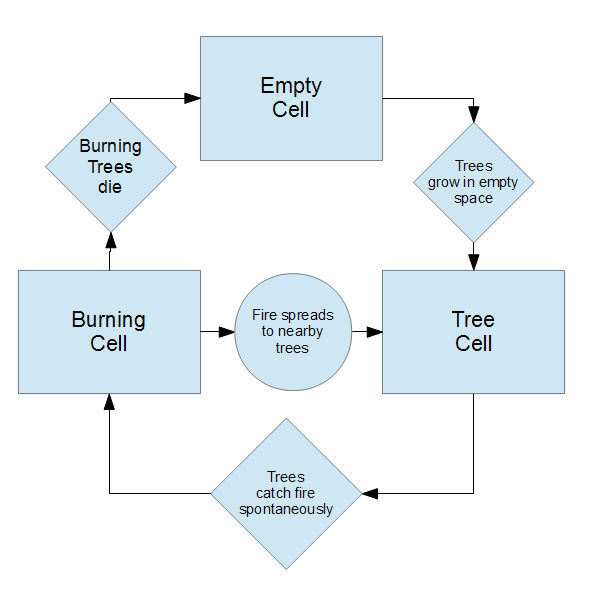
\includegraphics{tex/flowchart}

\newpage
\section{Implementation details}

The implementation was written in C, based on the student's past
experience with programming. The implementation did not require any complex
programming techniques, although a few key points are worth discussing.\\

As much of this simulation relies on probabilities, the use of a random number
generator requires some thought. the \texttt{random()} function of the C
standard library was selected due to its ease of use and availability, but as
it is only a pseudo-random number generator, perhaps this could be changed in
later efforts. There are websites that provide "true randomness" based on
atmospheric noise\cite{random}, and perhaps data from this service could be
used and compared against the output of \texttt{random()}.\\

Exporting the output of the program was done via the use of
libpng\cite{libpng}, which can easily convert 2d arrays into pictures. Sample
code was used from a third party website in order to assist with this
process\cite{png}. After each timestep was completed, the grid of cells was
exported to an image, with pixels being coloured based on their status.

\newpage
\section{Verification of program's output}

The implementation currently uses \texttt{random()} for its random number
generation, and this can be made deterministic by using a predefined seed with
the \texttt{srandom()} function. This will be used to compare the results of
later optimisations and multiprocessing techniques.

\newpage
\section{Algorithm's performance while scaling with forest size}

As the algorithm operates on neighbours, which remain constant with an
increasing grid size, performance should scale linearly with number of cells in
the grid.

\begin{verbatim}

$ time ./forest 100 0 100
real    0m1.179s
user    0m0.433s
sys     0m0.046s

$ time ./forest 200 0 100
real    0m2.524s
user    0m1.802s
sys     0m0.113s

$ time ./forest 300 0 100

real    0m5.395s
user    0m4.500s
sys     0m0.172s



\end{verbatim}

\newpage
\section{Further Considerations}

\newpage

\chapter{Optimisation and Parallel Implementation}

\newpage

\section{Optimisation of Serial Algorithm}

Before commencing with parallelisation of the \texttt{forest} program, the code
was examined for optimisations that could be made. An initial profile of the
program\footnote{The program was compiled without any optimisation flags, and
run on a 400 by 400 cell grid for 1000 timesteps.} with the \texttt{gprof} tool gave the following output:

\begin{verbatim}
Flat profile:

Each sample counts as 0.01 seconds.
  %   cumulative   self              self     total
 time   seconds   seconds    calls  ms/call  ms/call  name
 51.29      6.30     6.30     1000     6.30     8.04  out_png
 28.22      9.77     3.47 160000000     0.00     0.00  cell_auto
  8.32     10.79     1.02     1000     1.02     1.38  save_png_to_file
  6.28     11.57     0.77     1000     0.77     4.24  timestep
  5.83     12.28     0.72 320000000     0.00     0.00  pixel_at
  0.29     12.32     0.04                             print_usage
  0.00     12.32     0.00        1     0.00     0.00  alloc_forest
  0.00     12.32     0.00        1     0.00     0.00  parse_args

\end{verbatim}

This profile showed that approximately 65\% of execution time was spent
creating the PNG images and writing them to disk.\\

From this profile, two immediate conclusions were drawn: There should be an
alternate output method that does not incur any I/O overhead, and the PNG
output module should be optimimised.\\

a ``null'' output module was implemented, which allowed for benchmarking of the
code without worrying about the performance of third party libraries or I/O.
Terminal output via the \texttt{ncurses} library was also implemented, for easy
examination of code output changes.\\

The \texttt{timestep()} function was later moved into \texttt{main()} to save
unnecessary function call overhead.
\newpage
\subsection{PNG Module}

Inside the PNG module, several immediate optimisations were recognised: the
simple function \texttt{pixel\_at()} could be easily inlined, and the
intermediary struct \texttt{bitmap} was unnecessary and could be bypassed
completely. The module was rewritten and showed a considerable
performance increase:


\begin{verbatim}
Flat profile:

Each sample counts as 0.01 seconds.
  %   cumulative   self              self     total
 time   seconds   seconds    calls  ms/call  ms/call  name
 51.53      5.11     5.11     1000     5.11     5.11  out_png
 40.72      9.15     4.04 160000000     0.00     0.00  cell_auto
  7.88      9.93     0.78     1000     0.78     4.82  timestep
  0.10      9.94     0.01                             main
  0.00      9.94     0.00        1     0.00     0.00  alloc_forest
  0.00      9.94     0.00        1     0.00     0.00  parse_args

\end{verbatim}

As can be seen from the above profile, the rewritten \texttt{out\_png()}
function takes approximately 5ms per call, as opposed to 8ms in the original
version. The overhead from unnecessary function calls was removed by combining
procedures into one function, and the total execution time spent on output was
now 51\%, down from 65\%.

\subsection{Memory Allocation}

Initially, the two-dimensional grid that was used to store cell data was
allocated using three tiers of pointers: a top-level array containing double
pointers, inner arrays of pointers, and finally structs were allocated
individually.\\

This presented two problems: examining a cell would require four or even five
memory lookups to de-reference all the pointers, and with individually allocated
cell structs, the physical location of neighbouring cells in memory could be
quite distant, resulting in cache misses, particularly with larger grids.\\

By switching to a one-dimensional array that was allocated in one call to
\texttt{malloc()}, both of these problems were solved. Performance was shown to 
increase, although this was not measured as other optimisations took place
around this time.\\

\section{Parallelisation}

After the code was found to be sufficiently optimised in a serial environment,
methods to improve performance via parallelisation were investigated.\\

The main iteration loop over cells in the grid was reimplemented with two grids
instead of one, so that changes could be made to a "new" grid while reading an
"old" grid. This solved a problem with correctness in early versions of the
program, where fires would spread in one direction more than others, due to
examining neighbouring cells that were from the current timestep rather than
the previous timestep.\\

After moving to the two-grid implementation, iterating over one section of the
grid did not depend on other sections, and the loop could easily be
parallelised with OpenMP. Using MPI to further parallelise via domain
decomposition was also identified as a method to increase performance.

\subsection{OpenMP}

OpenMP allows for simple division of problems into smaller chunks which can be
processed independently. This is performed via multithreading.\\

OpenMP is implemented via the use of \texttt{pragma} directives added before
sections of code. To parallelise the main iteration loop in the \texttt{forest}
program, the \texttt{pragma omp parallel for} directive was added before the
loop initialisation, as follows:

\begin{verbatim}
    for (i = 0; i < f->simLength; i++) {
            #pragma omp parallel for
            for (x = 0; x < s; x++) {
                for (int y = 0; y < t; y++) {
                    int rand;
                    random_r(&stuff[omp_get_thread_num()], &rand);
                    cell_auto(f, x, y, f->oldGrid[(y * t) + x].status, &rand);
                    }
                }
\end{verbatim}

This split the loop at each row, giving each thread a row of the grid to
operate on.\\

Initial performance when using OpenMP showed a significant performance
decrease. Using the \texttt{OMP\_NUM\_THREADS} environment variable to limit
exectution to four threads showed more than a tenfold increase in execution time compared to
execution when using one thread:

\begin{verbatim}
$ export OMP_NUM_THREADS=1
$ time ./forest 400 400 null 1000
6.207 sec

$ export OMP_NUM_THREADS=4
$ time ./forest 400 400 null 1000
84.831 sec
\end{verbatim}

While examining the code, it was found that the \texttt{random()} function
used was not multithread-capable, as it relies on a global buffer to hold state
information between calls. However, the glibc library provides a reentrant random number
generator which is capable of being used in a multithreaded environment, called
\texttt{random\_r()}. The code was modified to use \texttt{random\_r()} with
individual state buffers for each thread, and performance was shown to scale
with threads:

\begin{verbatim}
$ export OMP_NUM_THREADS=1
$ time ./forest 400 400 null 1000
5.571 sec

$ export OMP_NUM_THREADS=2
$ time ./forest 400 400 null 1000
4.613 sec

$ export OMP_NUM_THREADS=4
$ time ./forest 400 400 null 1000
3.206 sec
\end{verbatim}

These tests were performed on a desktop computer with an Intel i7 2600k CPU.
When switching to a node on the Barrine cluster, performance still degraded
when using multiple threads:

\begin{verbatim}
forest with 400 x 400 grid on 1 threads took: 6.627 sec
forest with 400 x 400 grid on 2 threads took: 12.016 sec
forest with 400 x 400 grid on 4 threads took: 8.013 sec
forest with 400 x 400 grid on 8 threads took: 7.210 sec
\end{verbatim}

The cause of this performance decrease is as of yet unexplained, however it
could be due to differing CPU architectures. The Barrine node used has an Intel
Xeon L5520 CPU, which is from an earlier generation than the desktop CPU used.


\subsection{MPI}

Using MPI to parallelise programs involves running multiple instances of the
same program on multiple computers, or nodes, and communicating between each
node to transfer data. Each node running the MPI-enabled program is known as a
"rank".\\

A suitable method for improving performance with MPI would be to divide the
grid into multiple smaller sections, and have each rank process one section. At
the end of each timestep, each rank could pass their section to neighbouring
ranks, allowing an updated copy of the entire grid to exist on each rank. Then,
processing could continue. OpenMP could be used to divide the work on each rank
up into smaller subsections, allowing for all CPUs on a rank to be utilised
fully.\\

The MPI implementation of the program was written to use four ranks, each
working on one quarter of the grid. To keep implementation as simple as
possible, the entire grid was passed between ranks at the end of each timestep,
however it would also be possible to pass just the bordering rows/columns of
cells. This would keep transferred data to a minimum and improve performance,
but this technique was not able to be implemented in time.


\newpage
\section{Verification of implementation output}

To ensure that the program's output could be verified, it had to be able to
produce deterministic output. A verification output method was added, which
altered the seeding method for random number generation to use a static seed.
The module examines the contents of the cell grid at the final timestep of the
simulation, and produces an MD5 checksum of the contents. This was implemented
using glibc's \texttt{crypt()} function.\\

If the program's output can be determined at runtime, it should be possible to
reproduce the same output by running the program with the same arguments,
multiple times. This was found to be the case when using one OpenMP thread, but
when using multiple threads, the program's output changed between runs:


\begin{verbatim}

$ export OMP_NUM_THREADS=1
$ ./forest 240 240 verify 500
Grid checksum is: $1$cosc3500$Zz63shoT031bnGE.f1UVF/
$ ./forest 240 240 verify 500
Grid checksum is: $1$cosc3500$Zz63shoT031bnGE.f1UVF/
$ ./forest 240 240 verify 500
Grid checksum is: $1$cosc3500$Zz63shoT031bnGE.f1UVF/

$ export OMP_NUM_THREADS=2
$ ./forest 240 240 verify 500
Grid checksum is: $1$cosc3500$q.T.ss7LAG/oZpycVU9Ig0
$ ./forest 240 240 verify 500
Grid checksum is: $1$cosc3500$ibx89tXbp/9Jer53wZkPH.
$ ./forest 240 240 verify 500
Grid checksum is: $1$cosc3500$7R05CaitedeiVLqruuDFw0

\end{verbatim}

The reason for the non-determinism when using multiple threads is due to the
technique of pseudo-random number generators relying on a seed value and
producing random numbers in a sequence. When working in a single-threaded
context, one sequence is used over the entire grid - for example, a cell 
at position \textbf{n} in a grid would have the \textbf{n}\textsuperscript{th} 
number in a random sequence.\\

However, in a context where multiple threads are working on the same grid,
each thread requires its own sequence so as to avoid contention. This creates
the issue observed above. 

\newpage
\section{Test Plan}

The \texttt{forest} program's output should be made deterministic when working
with multiple threads, but once this has been accomplished, it can be run on
large grids for long simulation lengths.\\

One area which would be worthwhile exploring is the number of trees and burning
trees in a forest over time. As fires burn more rapidly when there are more
trees, it would be interesting to see the effect of fires that occur in
sparsely-populated forests, compared to densely populated forests. Collection
of these statistics is easily accomplished with the current program, and they
could be graphed using third-party software.

\newpage

\chapter{``Big Runs''}

\section{Performance Scaling on a HPC Cluster}

With an implementation that can be run on multiple computer nodes using MPI, as well as
being able to take advantage of multi-core CPUs with OpenMP, some consideration should be
given to performance when run on different configurations of threads and
ranks.\\

Because there is some overhead when synchronising between threads and ranks, it
is important to use a large grid size, so that there is sufficient work to be
done by each thread/rank between timesteps. Using a small grid size would
almost certainly result in the overhead generated by parallelisation
outweighing the benefits of the added processing power.\\

The OpenMP, MPI, and serial implementations were each run on a grid of
2560x1440 size, for 1000 timesteps. OpenMP-enabled implementations were each
run with 1, 2, 4, and 8 threads. the MPI implementation was fixed to 4 ranks
due to implementation restraints.\\
\\
\begin{tabular}{| l | l | l | l | l | l |}
\hline
Libraries used & OpenMP & MPI  & Total threads & Execution & \% \\
 & threads used & ranks used & & time  & \\ \hline
None & n/a & n/a & 1 & 113.661s & 100\% \\ \hline
OpenMP & 1 & n/a & 1 & 117.157s & 103\% \\ \hline
OpenMP & 2 & n/a & 2 & 204.803s & 180\% \\ \hline
OpenMP & 4 & n/a & 4 & 200.665s & 176\% \\ \hline
OpenMP & 8 & n/a & 8 & 139.342s & 122\% \\ \hline
MPI/OpenMP & 1 & 4 & 4 & 170.443s & 149\% \\ \hline
MPI/OpenMP & 2 & 4 & 8 & 171.454s & 150\% \\ \hline
MPI/OpenMP & 4 & 4 & 16 & 125.797s & 110\% \\ \hline
MPI/OpenMP & 8 & 4 & 32 & 120.502s & 106\% \\ \hline
\end{tabular}

\newpage
Unfortunately, it appears that the naive serial implementation is still faster
than all parallel implementations. As mentioned earlier, there is an overhead
when using OpenMP that was found to be absent when using a desktop CPU. This
may be the result of different OpenMP implementations or extra instructions
provided by newer-generation CPUs.\\

This demonstrates an issue with parallelisation that will become increasingly
important as computers begin to scale with core count, rather than with
clock speed. Parallelisation is not an ``easy fix'' that can be applied to
increase performance of any algorithm or procedure; it relies on careful
consideration and optimisation in order to provide benefits. Simply attempting
to give a program more CPUs will not increase its performance linearly, and in
many cases will reduce performance. Some algorithms cannot be parallelised, and
others may require too much overhead to be able to provide a performance
increase.\\

The \texttt{forest} program's algorithm should be able to benefit from
parallelisation in theory, but the implementation of MPI used includes large
amounts of unnecessary data transfer. This reduces the performance to a point
where the serial implementation is the best option to use, which should not be
the case.

\section{Testing Process Used}

The source package for the \texttt{forest} program includes a Makefile which
allows compilation with OpenMP or MPI functionality enabled. Also included are
PBS scripts to allow running of test runs with varying configurations of
MPI/OpenMP on a HPC cluster. These scripts also output the execution time of
each run.\\

\texttt{forest} has had a logging feature added. This allows the count of trees
and burning trees in the forest to be recorded in a text file at the end of
each timestep. This allows for the easy graphing of these numbers.\\

PBS jobs were submitted to the Savanna cluster, and execution times were
averaged over three runs, in order to account for CPU contention with other
jobs.\\

\newpage
\section{Scientific Experimentation}

Simulating forest fires is a potentially useful area of computer science,
because these fires are a large hazard in many countries, including Australia.
Learning how to control fires and understanding the safety features required to
protect people living in forest areas.\\

Unfortunately, many of the features that would be required to investigate these
areas were not implemented in \texttt{forest}. Much of the development cycle
was spent on parallelisation techniques, instead of improving the simulation.
However, the logging feature can be used to demonstrate the self-organised
criticality of the forest fire model:\\

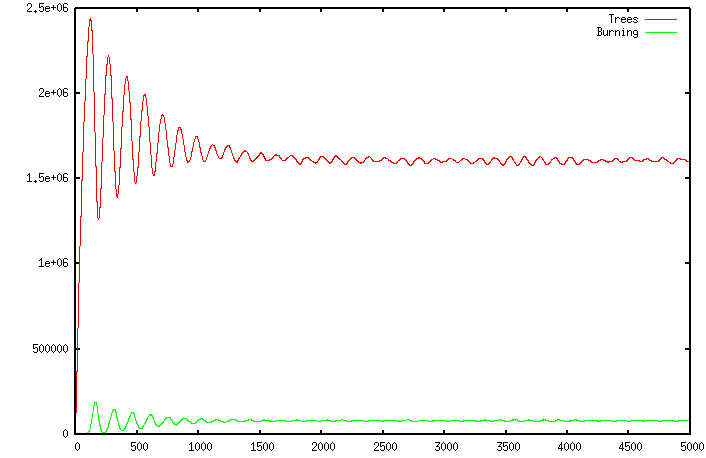
\includegraphics[scale=0.8]{tex/graph}


\newpage

\appendix
\chapter{Appendix One: Commands used during testing}

The following is a sample of the PBS job used during performance testing runs:
\begin{verbatim}
#!/bin/bash
#PBS -N mpi-test
#PBS -q workq
#PBS -A uq-COSC3500
#PBS -lwalltime=00:10:00
#PBS -lnodes=4:ppn=8
#PBS -lmem=1gb

. /usr/share/modules/init/bash

module load intel-mpi intel-cc-13

cd $PBS_O_WORKDIR
export TIMEFORMAT="%E sec"

export OMP_NUM_THREADS=8
export DIM=2560
export DIM2=1440
export LENGTH=1000

echo -n "forest with $DIM x $DIM2 grid for $LENGTH timesteps on
$OMP_NUM_THREADS threads using 4 MPI nodes took: " >&2
time mpirun -envall -np 4 forest-mpi $DIM $DIM2 null $LENGTH
\end{verbatim}

The following is a sample of the output of the previous job:
\begin{verbatim}
forest with 2560 x 1440 grid for 1000 timesteps on 8 threads WITHOUT MPI took:
139.342 sec
\end{verbatim}

\begin{thebibliography}{99}

\bibitem{png}
"Write a PNG file using C and libpng", 2010 Ben Bullock
http://www.lemoda.net/c/write-png/

\bibitem{libpng}
"libpng Home Page", 2013 Greg Roelofs
http://www.libpng.org/pub/png/libpng.html

\bibitem{random}
"RANDOM.ORG - True Random Number Service", 2012 RANDOM.ORG
http://www.random.org/

\end{thebibliography}
\end{document}
    
    
